\Author{\daAuthorTwo}

Since my research question "How can user-experience principals add to an intuitive map displayment for nonprofit activities in which people of different technical know-how levels collaborate?" is all about usability, I want to introduce you to its basic concepts and challenges but also provide some examples on how usability can impact a software's revenue and perception.

\blankLine

Usability is a critical aspect of software and interface design, ensuring that users can efficiently and effectively interact with a product or system. Its job is to provide clear feedback and "experiences" to the user, so interactions between software and human feel smooth and straight forward. Because each human being is different in its emotional experiences, it is difficult to design a kind of "one size fits all" solution. Due to this circumstance, many studies and experiments were conducted.
\autocite{Paul:Usability101}

\subsection{Why it is important}

Usability ensures that users can accomplish their goals with minimal frustration and maximum efficiency. With the increasing reliance on digital tools, usability plays a key role, not only, in shaping user experiences but also accessibility of software for diverse user groups. A well-designed and thought-out usability concept can go a long way from refining a once tedious and complicated to use product, to one that can be operated even by non-familiar users or disabled people. This plays a big part in the inclusion of all age and knowledge groups as well as the general market share through mass adoption because of the easiness.

\subsection{Components of Usability}

According to Jakob Nielsen, usability consists of five core components. To achieve the best possible usability, each of factors must be taken into account and be improved to its maximum.

\begin{itemize}
    \item Learnability
    \begin{description}
        \item How \textbf{easy} it is to accomplish basic tasks the first time  
    \end{description}

    \item Efficiency
    \begin{description}
        \item How \textbf{quickly} task can be accomplished after an initial learning period
    \end{description}

    \item Memorability
    \begin{description}
        \item How \textbf{memorable} actions are to users so, after an extended period of not using a software
    \end{description}

    \item Error handling
    \begin{description}
        \item How \textbf{many} errors users make while using the design and how \textbf{sever} they are  
    \end{description}

    \item Satisfaction
    \begin{description}
        \item How \textbf{pleasant} the overall experience of using the product is 
    \end{description}
\end{itemize}
\autocite{Paul:Usability101}

\blankLine

Now that we know these key points, what measures can we take to reach the goal of great usability? According to Nasrullah Hamidli, human-computer-interaction relies on consistency, visibility, feedback, and simplicity. Consistency ensures users do not need to learn new interactions for each task. For example, buttons should look alike and be in a similar location. This makes for a more natural navigation across the product and an overall familiar feel. Simplicity connects directly to this. Its goal is to minimize clutter and make user interfaces easy to understand and provide one, clear way to accomplish a task, not many possible, but complicated and unintuitive ways. It also aims to reduce distractions. Visibility allows users to clearly understand their options at any given moment, this is most often achieved through visual cues, like, grayed out buttons. This goes hand in hand with the feedback aspect, which provides immediate confirmation of actions. Loading indicators, color-changes and alike get used most often.

\blankLine

Another important part of designing a good UI are typography and colors. These
can act as parameters for the attention and emotions of users, as well as establish visual hierarchies, which, intern, contribute again to a simpler to navigate interface. 

\autocite{Paul:UIUXIntroduction}

\subsection{Fundamental concepts}

\textbf{Visual Hierarchy}

Visual hierarchy is a fundamental principle in UI/UX design that dictates how users perceive and navigate content. It ensures that important elements are more visually prominent, guiding users toward essential actions and information.

A bad design lacks differentiation in text size, weight, or spacing, making it hard to distinguish between headings, body text, and interactive elements for the user. This results in cluttered interfaces, increasing cognitive load and reduced usability.

\begin{figure} [H]
    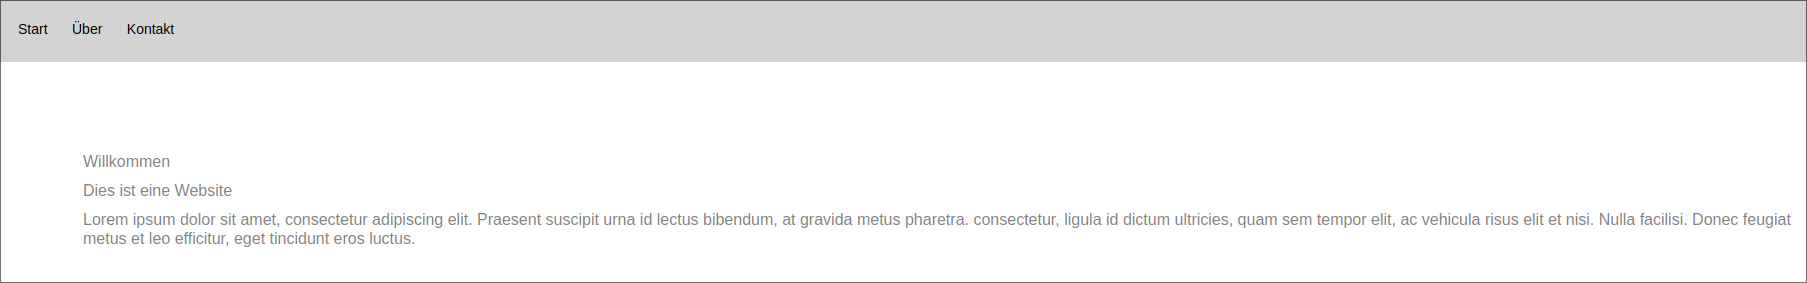
\includegraphics [width=1\textwidth] {images/paul/usabilityExamples/badVisualHierarchy.png}
    \caption{}
\end{figure}

A good design example effectively uses font size, color contrast, spacing, and alignment to distinguish primary content from secondary information. Headings are bold and larger, while body text is appropriately sized for readability. Proper spacing and alignment create a structured and easy-to-follow interface.

Source: FMD University - UX Visual Hierarchy

\blankLine

\textbf{Color Theory \& Contrast}

Color selection plays a critical role in usability and aesthetics. High contrast improves readability, while poor color choices can make content inaccessible, especially for users with visual impairments.

A bad design example features low-contrast elements, such as light gray text on a white background, making it difficult to read, especially for users with low vision or color blindness.

A good design example follows WCAG (Web Content Accessibility Guidelines) by ensuring high contrast between text and background. Colors are chosen deliberately to create visual harmony while maintaining functionality.

Source: Atmos - Color Theory in UI Design

\textbf{Consistent Layout \& Interaction Patterns}

Consistency in design enhances user experience by ensuring that UI elements and interactions are predictable across different screens.

A bad design example includes an inconsistent navigation bar where the position and style change across different screens, leading to confusion and frustration.

A good design example maintains a uniform layout with clearly defined navigation menus, button styles, and form elements. This consistency improves usability and allows users to develop mental models of how the system operates.

Source: Maze - UI Design Principles

\textbf{Button Placement \& Behavior}

Buttons are critical interactive elements in UI design. Their placement and responsiveness affect usability and efficiency.

A bad design example places primary actions (e.g., "Submit") in less prominent areas, while secondary actions (e.g., "Cancel") are emphasized, leading to potential user errors.

A good design example ensures that primary actions are clearly distinguishable with appropriate sizing and positioning. Visual and tactile feedback, such as hover effects or state changes, confirm user interactions.

Source: Dribbble - Button UI Design

\textbf{Feedback \& Responsiveness}

Providing immediate and clear feedback enhances user confidence and prevents frustration.

A bad design example lacks feedback for user actions, such as clicking a button without visual confirmation, leaving users uncertain if their action was registered.

A good design example includes real-time feedback mechanisms like loading indicators, success messages, and animations to confirm user interactions.

Source: Dribbble - Feedback UI Design

\textbf{Form Design Best Practices}

Forms are a crucial aspect of digital interfaces. Their usability impacts user satisfaction and data collection efficiency.

A bad design example relies solely on placeholder text without persistent labels, making it difficult for users to recall input requirements once they start typing.

A good design example includes clearly visible labels, real-time validation messages, and appropriately spaced input fields, reducing user errors and improving accessibility.

Source: Medium - Form Design Best Practices

\subsection{Challenges in designing for a broad user spectrum}

Designing for a diverse user base requires the addressing of varying levels of experience, prior knowledge, cognitive abilities, and accessibility needs. Failure to account for these differences can lead to usability issues, preventing certain groups from effectively using a system. Designers must implement features such as adjustable text sizes, screen reader compatibility, and intuitive navigation to ensure accessibility for all users.

\blankLine

Interfaces should always be tailored to the needs and expectations of the end-user. This leads to challenges when the user-group is not clearly defined or consists of people with widely different backgrounds. For example elderly people often need further guidance when interacting with digital solutions than members of younger generations. This leads back to the core components of usability-design, interfaces need to be simple and unmistakable in their functionality. Failing to provide these core concepts will sooner or later result in a frustrated and shrinking user base. 
\autocite{Paul:UIUXIntroduction}

\blankLine

\todo{wenn zu wenig inhalt dann könnte man auch noch was schreiben wieso des so is und auf welchen psychologischen dingen des basiert}


\newpage